As was mentioned on the \emph{Future Directions} section in~\cite{fairness-ECA}, one of the goals in the roadmap is to implement CSMA/ECA in cheap commodity hardware.

This report gathers all the necessary software, equipment and procedures that led to the translation of CSMA/ECA into WMP-Editor~\cite{FLAVIA}\cite{WMP-code}. It is intended to anyone who is interested on playing with MAC protocols in real hardware.

\section{Flying through WMP's concepts} 

On the other hand, this report is not written as a survey or an explanation on the subject of Finite State Machines (FSM); and neither details the work of FSM as an abstraction level capable of modifying the default behavior of wireless network cards. Instead the reader will be introduced to the terms used in the documentation as well as how they are appreciated through the graphical interfaces of the different applications used along.

\subsection{Directing the behavior}

The WMP allows us to \emph{program} different MAC protocols through a user interface (UI). This interface is what will be called the WMP-Editor from now on. In the WMP-Editor you can build blocks and connect them to other blocks. Some of these blocks can be conditional blocks and redirect the instruction flow according to an evaluation. In turn, every connection between blocks can execute an \emph{action} that can admit \emph{parameters}.

In the WMP-Editor, blocks are \emph{states} of the MAC program waiting for some trigger to unleash further actions and redirect the flow towards another state. Figure~\ref{fig:WMP-EditorLayout} shows an overview of the workspace in WMP-Editor.

\begin{figure*}[htbp]
  \centering
  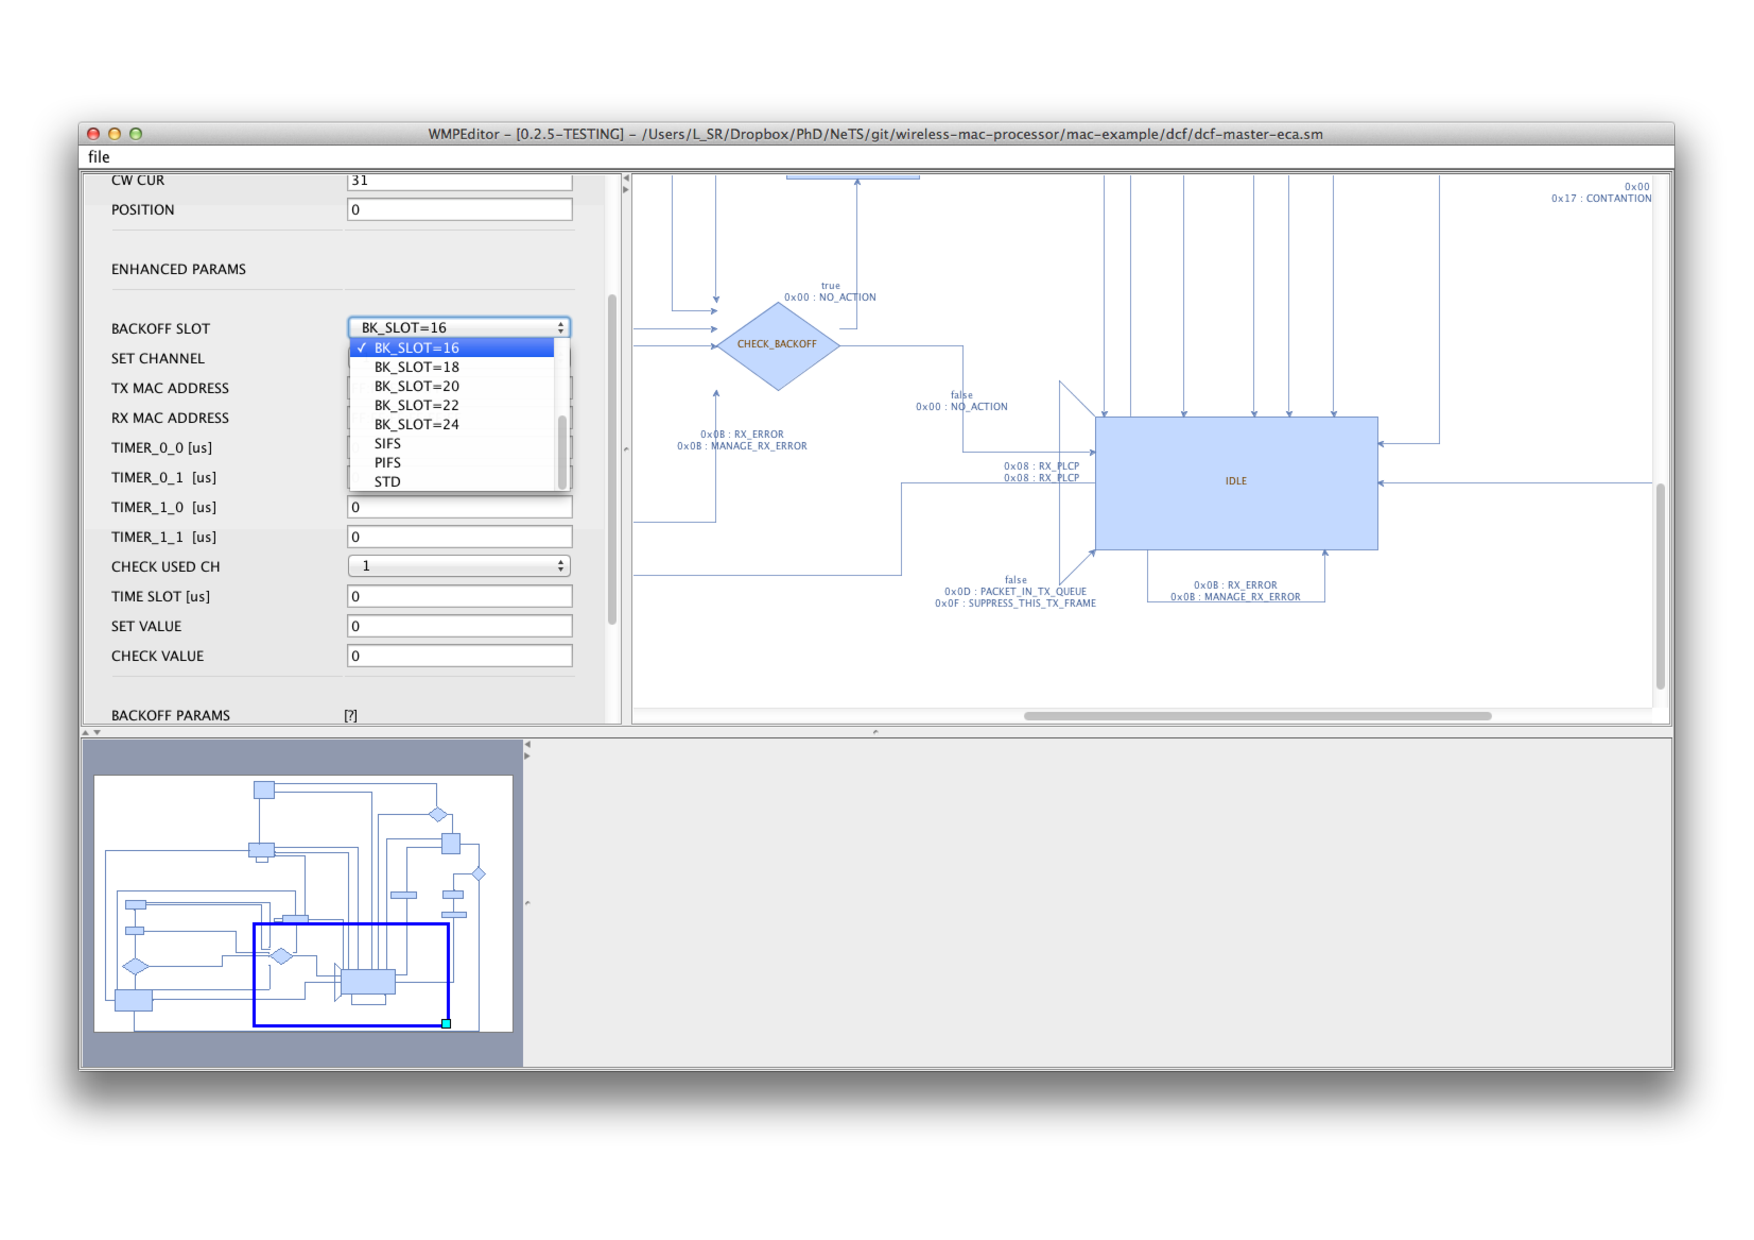
\includegraphics[width=0.95\linewidth]{figures/WMP-EditorLayout.pdf}
  \caption{WMP-Editor layout
  \label{fig:WMP-EditorLayout}}
\end{figure*}

When following the flow of an example state machine (like the one in Figure~\ref{fig:WMP-EditorLayout}), it is easy to see how arrows represent \emph{state changes}. These are the ones capable of executing actions during the state transitions. Figure~\ref{fig:WMP-EditorSetting}, shows how you can edit the parameter of action \texttt{0x0D TX\_PKT\_SCHEDULER} by using the drop-down menu on the left side (setting it to \texttt{BK\_SLOT=16}).

\begin{figure}[htbp]
  \centering
  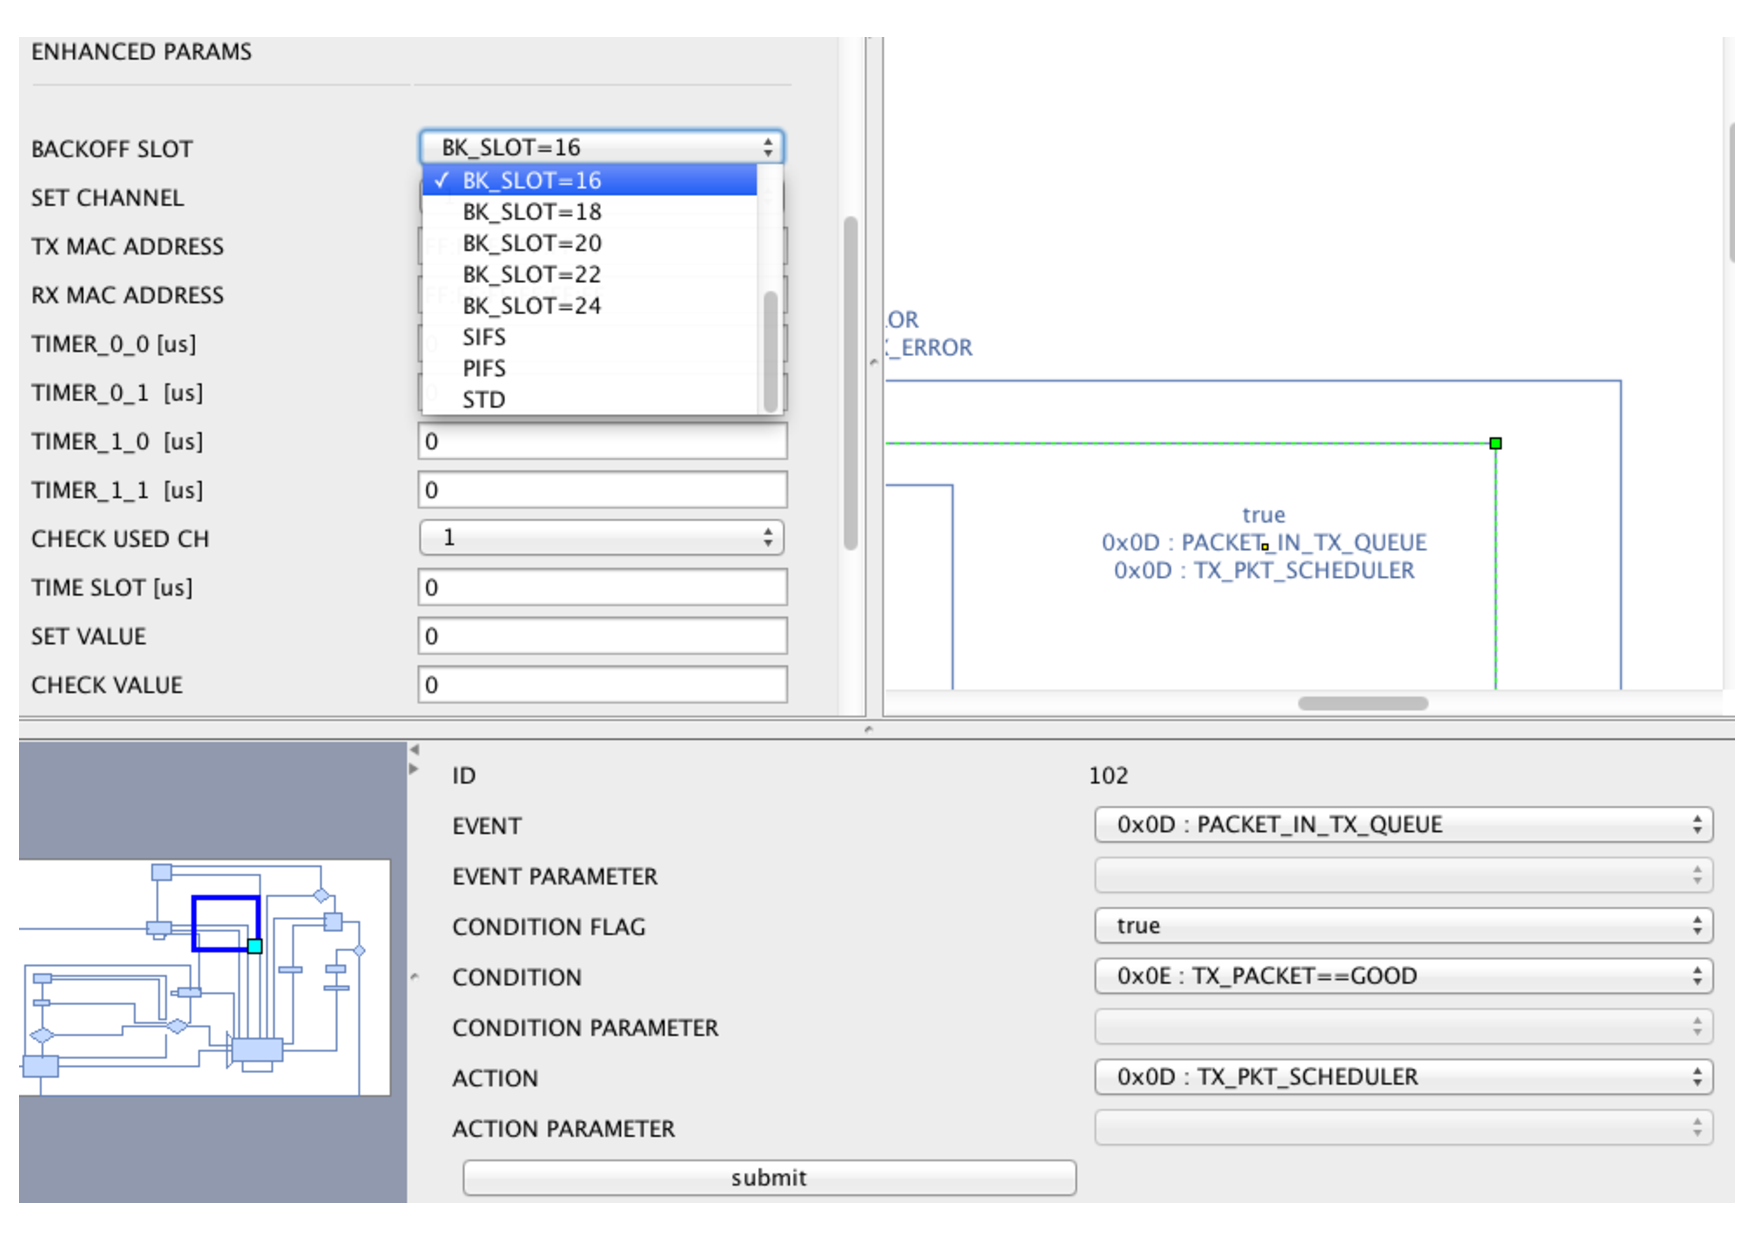
\includegraphics[width=0.95\linewidth]{figures/WMP-EditorSetting.pdf}
  \caption{Changing the parameter of action \texttt{0x0D TX\_PKT\_SCHEDULER}
  \label{fig:WMP-EditorSetting}}
\end{figure}